%diagram
\begin{center}
\begin{figure}[h]
	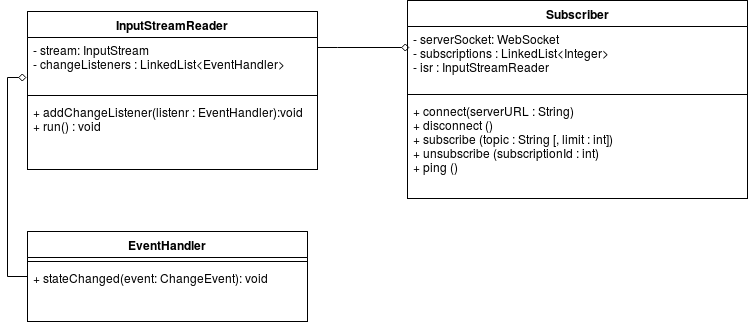
\includegraphics[width=15cm, height=7cm]{DataPull/DataPull.png}
\end{figure}
\end{center}
%description
With the android application we have to communicate with the zetta API platform and get streaming data and other data from the server.
\begin{itemize}
	\item Subscriber:\\
	Subscriber takes care of client-to-server communication using the zetta protocol for each. It makes use of the publish-subscribe model for data streaming. You can connect/disconnect and subscribe/unsubscribe to individual datastreams.

	\item InputStreamReader:\\
	The InputStreamReader is a runnable class so that it can be run by the subscriber class. It takes an inputstream from the server and you can addChangeListeners to cater to each different message the server sends. There is a LinkedList of event handlers that are called with a chain of responsibility.

	\item EventHandler:\\
	An EventHandler can be used by the InputStreamReader so that it can handle each event that the server sends.

\end{itemize}
%design patterns
Chain of Responsibility is used as a design pattern because it suits handling events from the server.
